\documentclass[12pt,a4paper]{article} 
\usepackage{graphicx}
\usepackage[portuguese]{babel}
\usepackage[applemac]{inputenc}
\usepackage[T1]{fontenc}
\usepackage{fullpage}

\title{Linguagens e Compiladores - Compilador L�xico} 
\author{Felipe Giunte Yoshida N$^o$USP 4978231\\Mariana Ramos Franco N$^o$USP 5179364}
\date {24 de Setembro de 2009}

\begin{document} 

\begin{figure}[!t]
\centering 

\includegraphics[width=15.5cm]{logo.pdf}
\end{figure}

\maketitle 

\section{Introdu��o}

A fun��o b�sica desta etapa do compilador � receber o c�digo fonte e dividi-lo em tokens. Para tal, foi sugerido pelo professor a cria��o de um aut�mato finito determin�stico (AFD), que recebe caracter por caracter o c�digo fonte, o ``quebra'' em tokens e monta uma tabela que identifica alguns tipos de token.

Inicialmente tentamos realizar a tarefa na linguagem C, mas devido a problemas de compatibilidade de bibliotecas entre Unix/Linux e Windows, resolvemos abandonar tal abordagem e reescrever o programa em Java, o que no final se mostrou mais organizado e pr�tico.

\section{Estruturas}

Para facilitar a estrutura��o do c�digo, criamos as seguintes estruturas:

\begin{itemize}
\item{AFD} - Aut�mato finito determin�stico, composto de estados e o estado ativo
\item{Estado} - Estado e suas transi��es
\item{Transicao} - Entradas que ativam uma transi��o e o estado que � ativado
\item{Token} - Parte do c�digo, que � classificada
\item{FluxoTokens} - Seq��ncia de tokens
\item{TabelaSimbolos} - Tabela auxiliar, usada na classifica��o dos tokens
\item{Simbolo} - Entrada da tabela de s�mbolos
\item{Tipo} - Classifica��o dos tipos de token
\item{PalavrasReservadas} - Defini��o das palavras reservadas
\end{itemize}

\section{L�gica}

Podemos dividir a parte l�gica desta etapa em basicamente duas partes:

\paragraph{Montador do aut�mato} Descrito na classe \emph{MontaAFD}, ele recebe um arquivo XML com a especifica��o do AFD abaixo, e o converte na estrutuda \emph{AFD}.

\begin{figure}[!ht]
\centering 
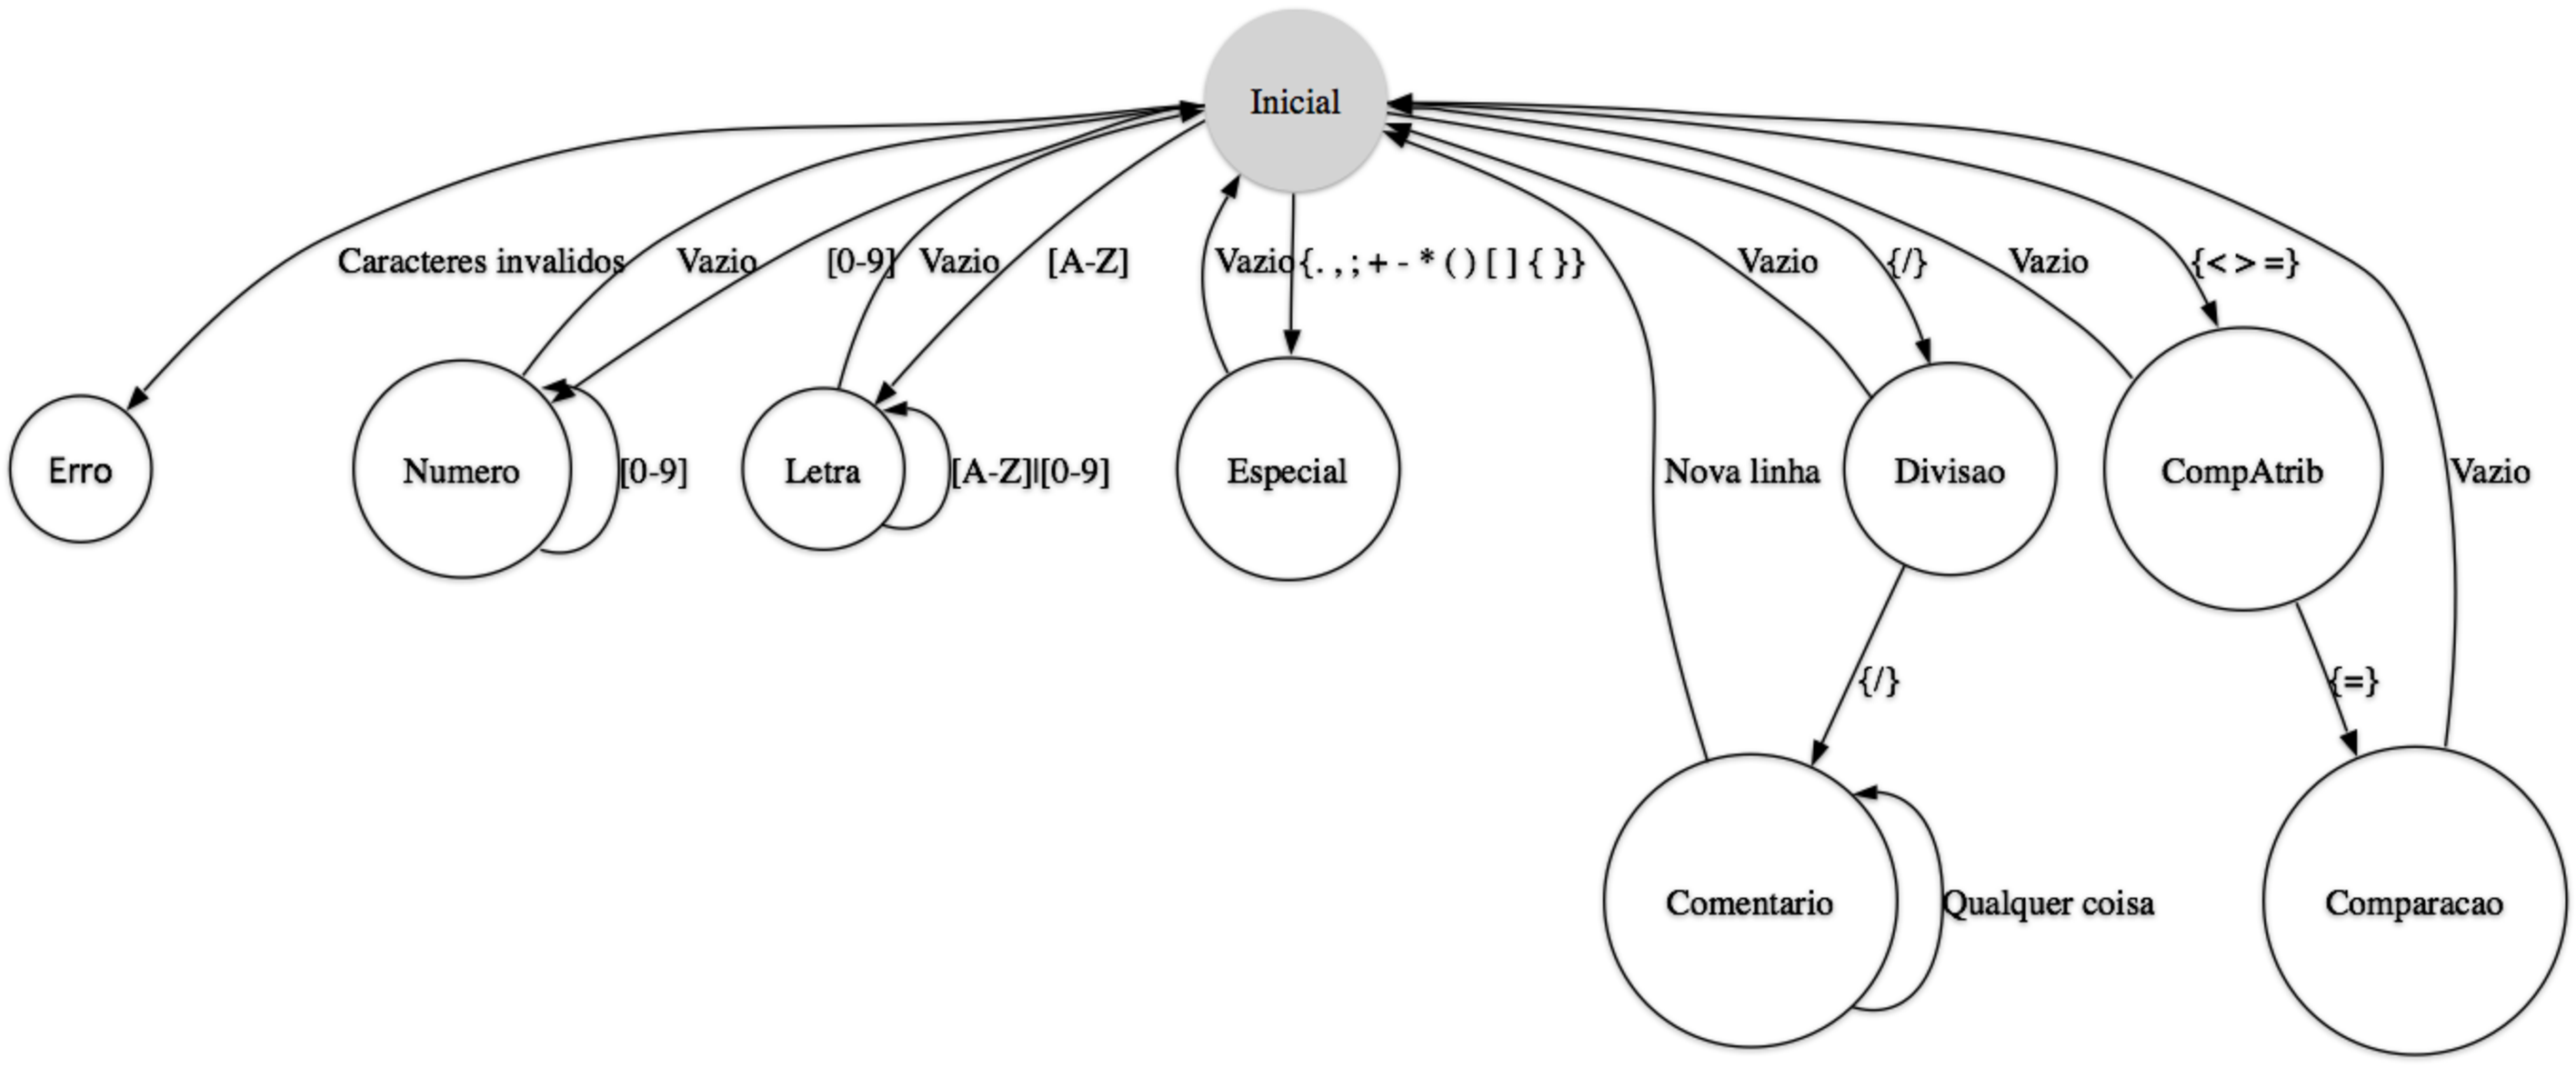
\includegraphics[width=15.5cm]{afd.pdf}
\end{figure}

\paragraph{Simulador do aut�mato} Descrito na classe \emph{PercorreAFD}, simula um AFD a partir do aut�mato montado no passo anterior e do c�digo fonte, que � analisado caracter por caracter.

\end{document} 